%\newpage\Large\mathphyssubsubsec{Lehramt Physik}\small
\section{50\%-Bachelor Physik (Lehramt)} % oder: physik-Lehramt?

Der 50\%-Bachelorstudiengang Physik ersetzt ab dem Wintersemester 15/16 den Physik-Lehramtsstudiengang. Er hat einerseits die Aufgabe, die notwendigen fachlichen Kompetenzen für den Physikunterricht beizubringen und den Übergang zum Master of Education zu ermöglichen. Andererseits soll ein Übergang in den Physik-Masterstudiengang möglich sein. Es ist unausweichlich, dass der so entstehende Studiengang für keinen der beiden Wege die optimale Lösung darstellt. Dennoch versucht der Studiengang, diese Bedingungen irgendwie umzusetzen. Wie, wird im Folgenden vor diesem Hintergrund beschrieben.

\subsection{Fächerkombinationen}

Gemäß Prüfungsordnung darf der 50\%-Bachelor Physik mit allen anderen 50\%-Studiengängen an der Universität Heidelberg, die für einen Master of Education qualifizieren, kombiniert werden. Eine explizite Liste findet sich in Anlage 8 der Prüfungsordnung für den Physik-Bachelor (gemeinsame Prüfungsordnung für 100\%- und 50\%-Bachelor). Unabhängig von der Fächerkombination darf am Ende dieses Studiums die Bachelorarbeit in Physik geschrieben werden. Allerdings ist die Kombination mit Mathematik zu empfehlen, da nur so die notwendigen mathematischen Grundlagen erworben werden können, siehe dazu Abschnitt „Mathematische Grundlagen“.

\subsection{Arbeitspensum}

Wie erwähnt muss der 50\%-Bachelor Physik für den Physik-Master qualifizieren. Dies heißt, dass die grundlegenden Vorlesungen Experimentalphysik 1-5 und Theoretische Physik 1-4 verpflichtend vorgeschrieben und in den ersten fünf, bzw. vier Semestern gehört werden müssen. Dies führt besonders in den ersten beiden Semestern zu einem hohen Arbeitspensum: Ist das zweite Fach beispielsweise Mathematik, so müssten im ersten Semester die Vorlesungen Experimentalphysik (Ex) 1, Theoretische Physik (Theo)\footnote{„Theo“ kann zu Verwirungen mit Informatikern führen, da diese das als „Theoretische Informatik“ verstehen} 1, Analysis (Ana) 1 und Lineare Algebra (LA) 1 gehört werden. Zum Vergleich: Für den 100\%-Bachelor Physik sieht die Fakultät 3 Vorlesungen dieses Umfangs pro Semester als angemessen an.

Im alten Lehramtsstudiengang wurde daher die Empfehlung ausgesprochen, die Vorlesungen der Theoretischen Physik um ein Jahr nach hinten zu schieben -- Theo 4 war damals aber nicht verpflichtend, sodass dies nicht zur Überschreitung der Regelstudienzeit von 6 Semestern führte. Für Studierende, die nicht auf BAföG (das nach der Regelstudienzeit gewöhnlich nicht mehr gezahlt wird) angewiesen sind, kann es auch weiterhin eine Option sein, Vorlesungen aus den ersten beiden Semestern aufzuschieben. Zu beachten ist allerdings, dass die in der Vorlesung Theo 1 behandelten Mathematischen Methoden in den Experimentalphysikvorlesungen verwendet werden. Zudem beträgt die Höchststudiendauer 9 Semester, nach denen man (außer nach Härtefallantrag) automatisch exmatrikuliert wird.

Die Semester 3-6 sind vom Arbeitsaufwand etwas geringer und außerdem hat man sich da dann schon an das Lernen an der Universität gewöhnt. Dabei ist stets der Großteil der Arbeit auf die Vorlesungszeit konzentriert, während in der vorlesungsfreien Zeit (abgesehen von Praktika) nicht viel geschieht.

Ziel dieses Abschnittes ist es sicherlich nicht, euch zu verunsichern oder gar Angst zu machen. Es ist durchaus problemlos möglich, die Vorlesungen wie vorgesehen zu absolvieren und mit guten Noten zu bestehen. Dies erfordert aber über das Semester hinweg disziplinierte Arbeit an den Übungszetteln für alle vier Vorlesungen. Die Erfahrung zeigt, dass es Studierende gibt, die mit diesem Arbeitspensum überlastet sind und dazu übergehen Übungsaufgaben abzuschreiben und so ins Hintertreffen geraten. Für ebenjene sei die Option aufgezeigt, dass es möglich ist, beispielsweise die Vorlesung Analysis 1, oder möglicherweise Theoretische Physik 1 um ein Jahr zu verschieben und so in der Lage zu sein, sich auf die verbleibenden drei Vorlesungen zu konzentrieren. Wir als Fachschaft, wie auch andere Anlaufstellen, stehen gerne als Ansprechpartner bereit, um bei derartigen Fragestellungen von unseren Erfahrungen zu berichten und Ratschläge zu geben.

\subsection{Mathematische Grundlagen}

„Mathematik ist die Sprache der Physik“ -- heißt es so schön und ist in der Tat korrekt. Man könnte sogar weiter gehen und sagen, dass die Menschheit nur deshalb begonnen hat, Mathematik zu betreiben, weil sich damit die Natur beschreiben lässt. Dies heißt aber auch, dass alle, die Physik betreiben -- sei es an Schulen, Universitäten oder in der Wirtschaft -- ein Grundverständnis für Mathematik benötigen. Für diejenigen unter euch, die Mathematik als zweites Fach gewählt haben, ist das Folgende nicht relevant, da die dort vorgesehenen Mathematik-Vorlesungen sicher mehr als nur ein Grundverständnis für Mathematik beibringen. Für alle anderen ist es aber vor gewisser Wichtigkeit.

Vieles der Mathematik, die in den ersten Semestern gebraucht wird, wird in den Physik-Vorlesungen behandelt. Grund dafür ist, dass die Fakultät für Mathematik und Informatik die Inhalte ihrer Vorlesungen natürlich an ihren eigenen Zielen und nicht denen des Physik-Studienganges ausrichtet. So beinhaltet beispielsweise die Vorlesung Theo 1 einen großen Mathematik-Teil, in dem beispielsweise die Lösung von Differentialgleichungen behandelt wird.

Allerdings sind nicht ohne Grund für den 100\%-Bachelorstudiengang Physik die Vorlesungen LA 1 sowie wahlweise Höhere Mathematik für Physiker (HöMa) 2\,\&\,3 oder Ana 2\,\&\,3 vorgeschrieben. Wichtige mathematische Konzepte wie Fouriertransformation werden in HöMa und Ex zeitgleich behandelt und die theoretische Beschreibung der Quantenmechanik ist ohne Kenntnis über Eigenvektoren aus LA 1 nicht zu verstehen. Das Beste wäre also, wenn all jene, die nicht Mathematik als zweites Fach gewählt haben, zumindest LA 1 vor Theo 4 hören (oder ein Buch lesen) würden. Besser sogar LA 1 und HöMa 2\,\&\,3 oder Ana 2\,\&\,3. Diese Vorlesungen sind im Modellstudienplan allerdings nicht vorgesehen, wodurch dies quasi freiwillige Zusatzarbeit wäre. Wie schon erwähnt könnte man auch hier in Erwägung ziehen, gewisse Vorlesungen aufzuschieben, um die notwendigen Mathematikkenntnisse vorher zu erlangen.


\subsection{Interdisziplinäres Modul}

Um denjenigen, die das Ziel haben, mit einem Fachmaster nach dem 50\%-Bachelorstudiengang fortzufahren, die Pflicht zu nehmen, Module in den Bildungswissenschaften zu absolvieren, sieht der 50\%-Bachelor Physik vor, dass man die Entscheidung zwischen Fachmaster und Master of Education schon im 5. Semester trifft. In 5.\,\&\,6. Semester kann man nämlich zwischen besagten Modulen in den Bildungswissenschaften auf der einen Seite (Lehramtsoption) und Praktika und Seminar auf der anderen Seite (interdisziplinäre Option) wählen. Ersteres ist notwendig für die Zulassung zum Master of Education, zweites zielt auf einen Fach-Master ab. Genauer ist dies in Anlage 9 Der Prüfungsordnung beschrieben.


\subsection{Zulassung zum Master Physik}

Dies Zulassungsordnung des Masterstudiengang Physik ist sehr freundlich gegenüber Studierenden. Es wird als Voraussetzung lediglich ein Anteil von 50\% Physik-relevanter Inhalte im Bachelorstudium gefordert. Dies ist gewährleistet, wenn man die Bachelorarbeit in Physik schreibt und die zuvor beschriebene interdisziplinäre Option wählt. Einer Zulassung zum Physik-Master steht damit nichts im Wege.

\begin{figure}[h] %Nur falls Bild auf gleicher Seite wie letzter Absatz. %TODO:Layout
\centering{
    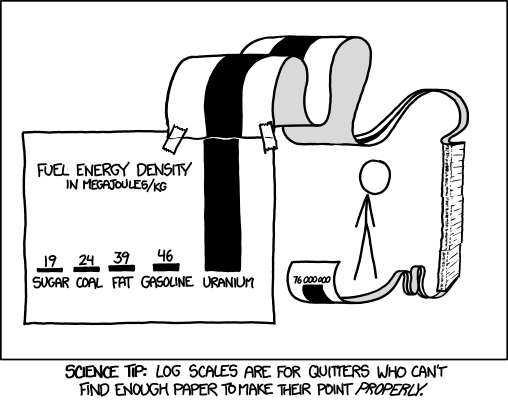
\includegraphics[width=\textwidth]{bilder/log_scale.png}
}
\end{figure}

%TODO: noch ein Modellstudienplan oder so einfügen.


%TODO: PO Anlage 7-9 !!!
